%% SECTION HEADER /////////////////////////////////////////////////////////////////////////////////////
\section{Convergence tests of the solution}
\label{sec:convergence}

%% SECTION CONTENT ////////////////////////////////////////////////////////////////////////////////////

\subsection{Spatial convergence}
Spatial convergence was determined after simulations for samples with elements of different order of the Legendre polynomial (see Eq. \ref{eq:nodes}).
The polynomial order for the \(\xi\times \eta\) plane in the local reference system were changed in the set: \(p=[4,\,5,\,7,\,9,\, 11]\).
The exact order was assumed for each component to minimise the non-zero value of coupling matrix \(\textbf{G}\).
Due to the perpendicularity of the core elements to the skin, the nodes along the core thickness are fixed to 5.
As a criterion for convergence, the percentage error defined as:
\begin{eqnarray}
	\delta^{\mathrm{conv}} = \frac{\sum{\left(e^{\mathrm{max}}-e^{p}\right)^2}}{\sum{\left(e^{max}\right)^2}} \times 100\%,
	\label{eq:perc_err_conv}
\end{eqnarray}
where \(e^{max}\) and \(e^{p}\) are the signal envelopes for the case with the elements of \(11^{\mathrm{th}}\) polynomial order and the observed case, respectively.
A 5\% threshold was assumed for choosing the degree of the polynomial.
The signal envelope is obtained using the Hilbert transform, which is defined as \cite{staszewski2004health}:
\begin{eqnarray}
	\label{eq:hilbert}
	\hat{x}(t) &=& \frac{1}{\pi}\int_{-\infty}^{+\infty}x(\tau)\frac{1}{t-\tau}\diff\tau,\\
	\label{eq:envelope}
	e(t) &=& \sqrt{x^2(t)+\hat{x}^2(t)}.
\end{eqnarray}
\nomtypeD[e]{\(e(t)\)}{Signal envelope}{}%
\nomtypeR[t]{\(t\)}{Time vector}{}{\unit{\second}}%

The example of the simulated signals of 100 \unit{\kHz} are presented in Fig. \ref{fig:dx_conv}\textbf{(a)}.
It can be seen that despite the good agreement of the wave speed for all cases, the amplitudes converge only for a polynomial of order 7.
Based on the graph showing simulation errors (Fig. \ref{fig:dx_conv}(\textbf{b})), the polynomial of order \(p=7\) was selected for 50 and 100 \unit{\kHz} signals, and order \(p=9\) was selected for the 150 \unit{\kHz} signal.
 
Tab \ref{tab:elements_nodes} contains a complete list of elements with the number of nodes on each axis \(\xi\times \eta \times \zeta\) which were assumed in simulations.
\begin{figure}[H]
	\begin{center}
		\includegraphics[width=0.95\textwidth]{Chapter_5/dx_conv}
	\end{center}
	\caption{Spatial convergence for the sample, \textbf{(a)} the sensor signals of 100 \unit{\kHz} for various number of the in-plane nodes (\(n \times m\)) of the element, \textbf{(b)} percent error for the differ polynomial order}
	\label{fig:dx_conv}
\end{figure}
\begin{table}[H]
	\small
	\tabcolsep=0.5cm
	\centering
	\caption{\label{tab:elements_nodes}The node numbers of the sample components.}
	\begin{tabular}{cccc}
		\toprule
		\multirow{3}{*}{\textbf{Component}} & \multicolumn{3}{c}{\textbf{Number of element nodes}}\\
		& \multicolumn{3}{c}{\(n\times m \times l\)}\\
		& 50 \unit{\kHz} & 100 \unit{\kHz} & 150 \unit{\kHz}\\
		\midrule
		Core & \multicolumn{2}{c}{\numproduct{8 x 5 x 1}} & \numproduct{10 x 5 x 1}\\
		Adhesive layer & \multicolumn{2}{c}{\numproduct{8 x 8 x 1}} & \numproduct{10 x 10 x 1}\\
		Skin & \multicolumn{2}{c}{\numproduct{8 x 8 x 4}} & \numproduct{10 x 10 x 1}\\
		Glue & \multicolumn{2}{c}{\numproduct{8 x 8 x 1}} & \numproduct{10 x 10 x 1}\\
		\ac{pzt} & \multicolumn{2}{c}{\numproduct{8 x 8 x 3}} & \numproduct{10 x 10 x 3}\\
		\bottomrule
	\end{tabular}
\end{table}

While the maximum length of the skin element is 6 \unit{\mm}, such a \ac{cfrp} model satisfies the condition of at least six nodes per wavelength for the \ac{a0}, as it is the shortest mode propagating in the assumed frequency range.
Table~\ref{tab:wavelength} shows the \ac{a0} wavelengths for various frequency and propagation angles.
\begin{table}[H]
	\small
	\tabcolsep=0.75cm
	%\centering
	\caption{\label{tab:wavelength}The wavelength of the \ac{a0} mode propagated in the presented \ac{cfrp} plate.}
	\begin{tabular}{cccccc}
		\toprule
		\textbf{Frequency} & \multicolumn{5}{c}{\textbf{Propagation angle}}\\
		\unit{\kHz} & \ang{0} & \ang{30} & \ang{45} & \ang{60} & \ang{90}\\
		\midrule
		50 & 16.5& 15.2&15.0&15.2&16.6\\
		100 & 10.3& 9.6&9.5&9.6&10.3\\
		\bottomrule
		\multicolumn{6}{r}{{\scriptsize{source: Dispersion Calculator v1.9}}}
	\end{tabular}
\end{table}
\subsection{Temporal convergence}
A temporal convergence test is conducted to select the appropriate time step value.
The critical value of time increment (\(\Delta t_{cr}\)) depends on the mesh size and the wave mode velocity.
If this value is set over (\(\Delta t_{cr}\)), the displacement of the structure will increase to infinity in the initial moments of the simulation as it is presented in Fig. \ref{fig:dt_cr}.
This indicates that the time step have to be further decreased which can be easy implemented for testing of the stability of the method.
\begin{figure}[!tbh]
	\begin{center}
		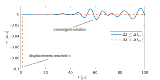
\includegraphics[width=0.95\textwidth]{Chapter_5/dt_cr}
	\end{center}
	\caption{The displacement of the plate at a point of 50 mm away from actuator in the case of correctly and incorrectly selected time increments.}
	\label{fig:dt_cr}
\end{figure}
